\chapter{Data and Methodology}
\label{chap:met}

\section{Raw Data}

	The data originates from two sources. The first and most important source is Thomson Reuters Datastream. It covers publicly traded shares from developed countries of Europe, Japan and Asia-Pacific (Australia, New Zealand, Hong Kong, and Singapore) and contains the firms' yearly accounting figures and daily market information (e.g., price and volume).  The second data source is Institutional Brokers’ Estimate System (I/B/E/S) from Wharton Research Data Services, which provides analysts' forecasts. 
	
	The firms are filtered based on [TODO add source of filtering methods].  
	The final sample includes 8350 companies.


\section{Anomalies Data}
	The anomaly dataset of OTMH (TODO cite) consists of 153 anomalies published in leading financial and accounting journals. The data is monthly and spans from January 1990 to December 2018. It covers the same 8350 firms as the raw data, totaling 1,607,117 observations. I choose 30 most important anomalies found in OTMH for my thesis.    
	
	The list of the anomalies can be found in the Appendix. [TODO]. 
	
	Table \ref{tab:descr} shows descriptive statistics of the anomalies data. [TODO fit too long fund table to page or split across multiple pages.]
		
	Figure \ref{fig:corrplot}, shows plot of the correlation matrix of the anomalies.

	Figure \ref{fig:hist_returns} shows histogram of monthly returns. 
	

	%\begin{tabular}{lrrrrrrrr}
\toprule
{} &      count &  mean &     std &     min &     25\% &     50\% &     75\% &    max \\
\midrule
Lagged Momentum                            &  1607088.0 &   0.0 &  0.0316 & -0.1518 & -0.0053 & -0.0009 &  0.0029 &  1.000 \\
Seasonality                                &  1607088.0 &  -0.0 &  0.0282 & -0.2622 & -0.0034 & -0.0002 &  0.0021 &  1.000 \\
Short-Term Reversal                        &  1607088.0 &  -0.0 &  0.2430 & -0.9831 & -0.1276 & -0.0178 &  0.1027 &  1.000 \\
Momentum-Reversal                          &  1607088.0 &   0.0 &  0.0200 & -0.0802 & -0.0054 & -0.0008 &  0.0029 &  1.000 \\
52-Week High                               &  1607088.0 &  -0.0 &  0.3316 & -1.0000 & -0.1828 &  0.0764 &  0.2445 &  0.678 \\
RD / Market Equity                         &  1607088.0 &  -0.0 &  0.0169 & -0.0311 & -0.0001 &  0.0000 &  0.0000 &  1.000 \\
Liquidity Shocks                           &  1607088.0 &  -0.0 &  0.0055 & -0.0016 & -0.0001 & -0.0001 & -0.0000 &  1.000 \\
Earnings Predictability                    &  1607088.0 &   0.0 &  0.0158 & -0.0081 & -0.0006 &  0.0000 &  0.0000 &  1.000 \\
Seasonality 6-10 A                         &  1607088.0 &  -0.0 &  0.0220 & -0.1208 & -0.0055 &  0.0000 &  0.0029 &  1.000 \\
Change in Common Equity                    &  1607088.0 &  -0.0 &  0.0153 & -0.0199 & -0.0013 & -0.0003 & -0.0001 &  1.000 \\
Seasonality 6-10 N                         &  1607088.0 &   0.0 &  0.0220 & -0.1307 & -0.0050 &  0.0000 &  0.0020 &  1.000 \\
Seasonality 2-5 N                          &  1607088.0 &   0.0 &  0.0219 & -0.1313 & -0.0061 & -0.0005 &  0.0035 &  1.000 \\
Seasonality 2-5 A                          &  1607088.0 &  -0.0 &  0.0180 & -0.1002 & -0.0042 & -0.0000 &  0.0027 &  1.000 \\
Leverage Component of Book/Price           &  1607088.0 &   0.0 &  0.0089 & -0.0057 & -0.0002 & -0.0001 & -0.0000 &  1.000 \\
Amihud's Measure (Illiquidity)             &  1607088.0 &   0.0 &  0.0221 & -0.0113 & -0.0005 & -0.0002 & -0.0001 &  1.000 \\
Profit Margin                              &  1607088.0 &   0.0 &  0.0652 & -1.0000 & -0.0000 &  0.0011 &  0.0097 &  1.000 \\
Volume Trend                               &  1607088.0 &   0.0 &  0.2040 & -0.8532 & -0.0873 &  0.0000 &  0.0979 &  1.000 \\
Coefficient of Variation of Share Turnover &  1607088.0 &  -0.0 &  0.1144 & -0.1469 & -0.0625 & -0.0279 &  0.0170 &  1.000 \\
Earnings Forecast-to-Price                 &  1607088.0 &   0.0 &  0.0137 & -0.1066 & -0.0006 &  0.0000 &  0.0000 &  1.000 \\
Duration of Equity                         &  1607088.0 &   0.0 &  0.0624 & -1.0000 & -0.0006 &  0.0000 &  0.0068 &  1.000 \\
Seasonality 11-15 N                        &  1607088.0 &   0.0 &  0.0213 & -0.1246 & -0.0032 &  0.0000 &  0.0005 &  1.000 \\
Operating Profits to Assets                &  1607088.0 &   0.0 &  0.0562 & -0.3581 & -0.0122 &  0.0000 &  0.0011 &  1.000 \\
Max                                        &  1607088.0 &   0.0 &  0.1913 & -0.2571 & -0.1111 & -0.0544 &  0.0416 &  1.000 \\
Whited-Wu Index                            &  1607088.0 &   0.0 &  0.1681 & -0.7012 & -0.0528 &  0.0000 &  0.0489 &  1.000 \\
Net Operating Assets                       &  1607088.0 &  -0.0 &  0.0171 & -0.0869 & -0.0007 & -0.0001 &  0.0000 &  1.000 \\
Accruals                                   &  1607088.0 &   0.0 &  0.0484 & -0.3996 & -0.0043 &  0.0000 &  0.0033 &  1.000 \\
Idiosyncratic Risk                         &  1607088.0 &  -0.0 &  0.1999 & -0.2929 & -0.1204 & -0.0539 &  0.0528 &  1.000 \\
Coskewness                                 &  1607088.0 &  -0.0 &  0.1996 & -1.0000 & -0.1014 &  0.0000 &  0.1074 &  1.000 \\
Liquidity Beta 5                           &  1607088.0 &  -0.0 &  0.0724 & -0.3288 & -0.0298 &  0.0000 &  0.0213 &  1.000 \\
Liquidity Beta 3                           &  1607088.0 &  -0.0 &  0.0568 & -0.3347 & -0.0100 &  0.0000 &  0.0204 &  1.000 \\
\bottomrule
\end{tabular}

	
	\begin{table}
		\resizebox{\textwidth}{!}{\begin{tabular}{lrrrrrrrr}
\toprule
{} &      count &  mean &     std &     min &     25\% &     50\% &     75\% &    max \\
\midrule
Lagged Momentum                            &  1607088.0 &   0.0 &  0.0316 & -0.1518 & -0.0053 & -0.0009 &  0.0029 &  1.000 \\
Seasonality                                &  1607088.0 &  -0.0 &  0.0282 & -0.2622 & -0.0034 & -0.0002 &  0.0021 &  1.000 \\
Short-Term Reversal                        &  1607088.0 &  -0.0 &  0.2430 & -0.9831 & -0.1276 & -0.0178 &  0.1027 &  1.000 \\
Momentum-Reversal                          &  1607088.0 &   0.0 &  0.0200 & -0.0802 & -0.0054 & -0.0008 &  0.0029 &  1.000 \\
52-Week High                               &  1607088.0 &  -0.0 &  0.3316 & -1.0000 & -0.1828 &  0.0764 &  0.2445 &  0.678 \\
RD / Market Equity                         &  1607088.0 &  -0.0 &  0.0169 & -0.0311 & -0.0001 &  0.0000 &  0.0000 &  1.000 \\
Liquidity Shocks                           &  1607088.0 &  -0.0 &  0.0055 & -0.0016 & -0.0001 & -0.0001 & -0.0000 &  1.000 \\
Earnings Predictability                    &  1607088.0 &   0.0 &  0.0158 & -0.0081 & -0.0006 &  0.0000 &  0.0000 &  1.000 \\
Seasonality 6-10 A                         &  1607088.0 &  -0.0 &  0.0220 & -0.1208 & -0.0055 &  0.0000 &  0.0029 &  1.000 \\
Change in Common Equity                    &  1607088.0 &  -0.0 &  0.0153 & -0.0199 & -0.0013 & -0.0003 & -0.0001 &  1.000 \\
Seasonality 6-10 N                         &  1607088.0 &   0.0 &  0.0220 & -0.1307 & -0.0050 &  0.0000 &  0.0020 &  1.000 \\
Seasonality 2-5 N                          &  1607088.0 &   0.0 &  0.0219 & -0.1313 & -0.0061 & -0.0005 &  0.0035 &  1.000 \\
Seasonality 2-5 A                          &  1607088.0 &  -0.0 &  0.0180 & -0.1002 & -0.0042 & -0.0000 &  0.0027 &  1.000 \\
Leverage Component of Book/Price           &  1607088.0 &   0.0 &  0.0089 & -0.0057 & -0.0002 & -0.0001 & -0.0000 &  1.000 \\
Amihud's Measure (Illiquidity)             &  1607088.0 &   0.0 &  0.0221 & -0.0113 & -0.0005 & -0.0002 & -0.0001 &  1.000 \\
Profit Margin                              &  1607088.0 &   0.0 &  0.0652 & -1.0000 & -0.0000 &  0.0011 &  0.0097 &  1.000 \\
Volume Trend                               &  1607088.0 &   0.0 &  0.2040 & -0.8532 & -0.0873 &  0.0000 &  0.0979 &  1.000 \\
Coefficient of Variation of Share Turnover &  1607088.0 &  -0.0 &  0.1144 & -0.1469 & -0.0625 & -0.0279 &  0.0170 &  1.000 \\
Earnings Forecast-to-Price                 &  1607088.0 &   0.0 &  0.0137 & -0.1066 & -0.0006 &  0.0000 &  0.0000 &  1.000 \\
Duration of Equity                         &  1607088.0 &   0.0 &  0.0624 & -1.0000 & -0.0006 &  0.0000 &  0.0068 &  1.000 \\
Seasonality 11-15 N                        &  1607088.0 &   0.0 &  0.0213 & -0.1246 & -0.0032 &  0.0000 &  0.0005 &  1.000 \\
Operating Profits to Assets                &  1607088.0 &   0.0 &  0.0562 & -0.3581 & -0.0122 &  0.0000 &  0.0011 &  1.000 \\
Max                                        &  1607088.0 &   0.0 &  0.1913 & -0.2571 & -0.1111 & -0.0544 &  0.0416 &  1.000 \\
Whited-Wu Index                            &  1607088.0 &   0.0 &  0.1681 & -0.7012 & -0.0528 &  0.0000 &  0.0489 &  1.000 \\
Net Operating Assets                       &  1607088.0 &  -0.0 &  0.0171 & -0.0869 & -0.0007 & -0.0001 &  0.0000 &  1.000 \\
Accruals                                   &  1607088.0 &   0.0 &  0.0484 & -0.3996 & -0.0043 &  0.0000 &  0.0033 &  1.000 \\
Idiosyncratic Risk                         &  1607088.0 &  -0.0 &  0.1999 & -0.2929 & -0.1204 & -0.0539 &  0.0528 &  1.000 \\
Coskewness                                 &  1607088.0 &  -0.0 &  0.1996 & -1.0000 & -0.1014 &  0.0000 &  0.1074 &  1.000 \\
Liquidity Beta 5                           &  1607088.0 &  -0.0 &  0.0724 & -0.3288 & -0.0298 &  0.0000 &  0.0213 &  1.000 \\
Liquidity Beta 3                           &  1607088.0 &  -0.0 &  0.0568 & -0.3347 & -0.0100 &  0.0000 &  0.0204 &  1.000 \\
\bottomrule
\end{tabular}
}
		\caption{Descriptive Statistics of the Anomalies}
		\label{tab:descr}
	\end{table}


	\begin{center}
		\begin{figure}
			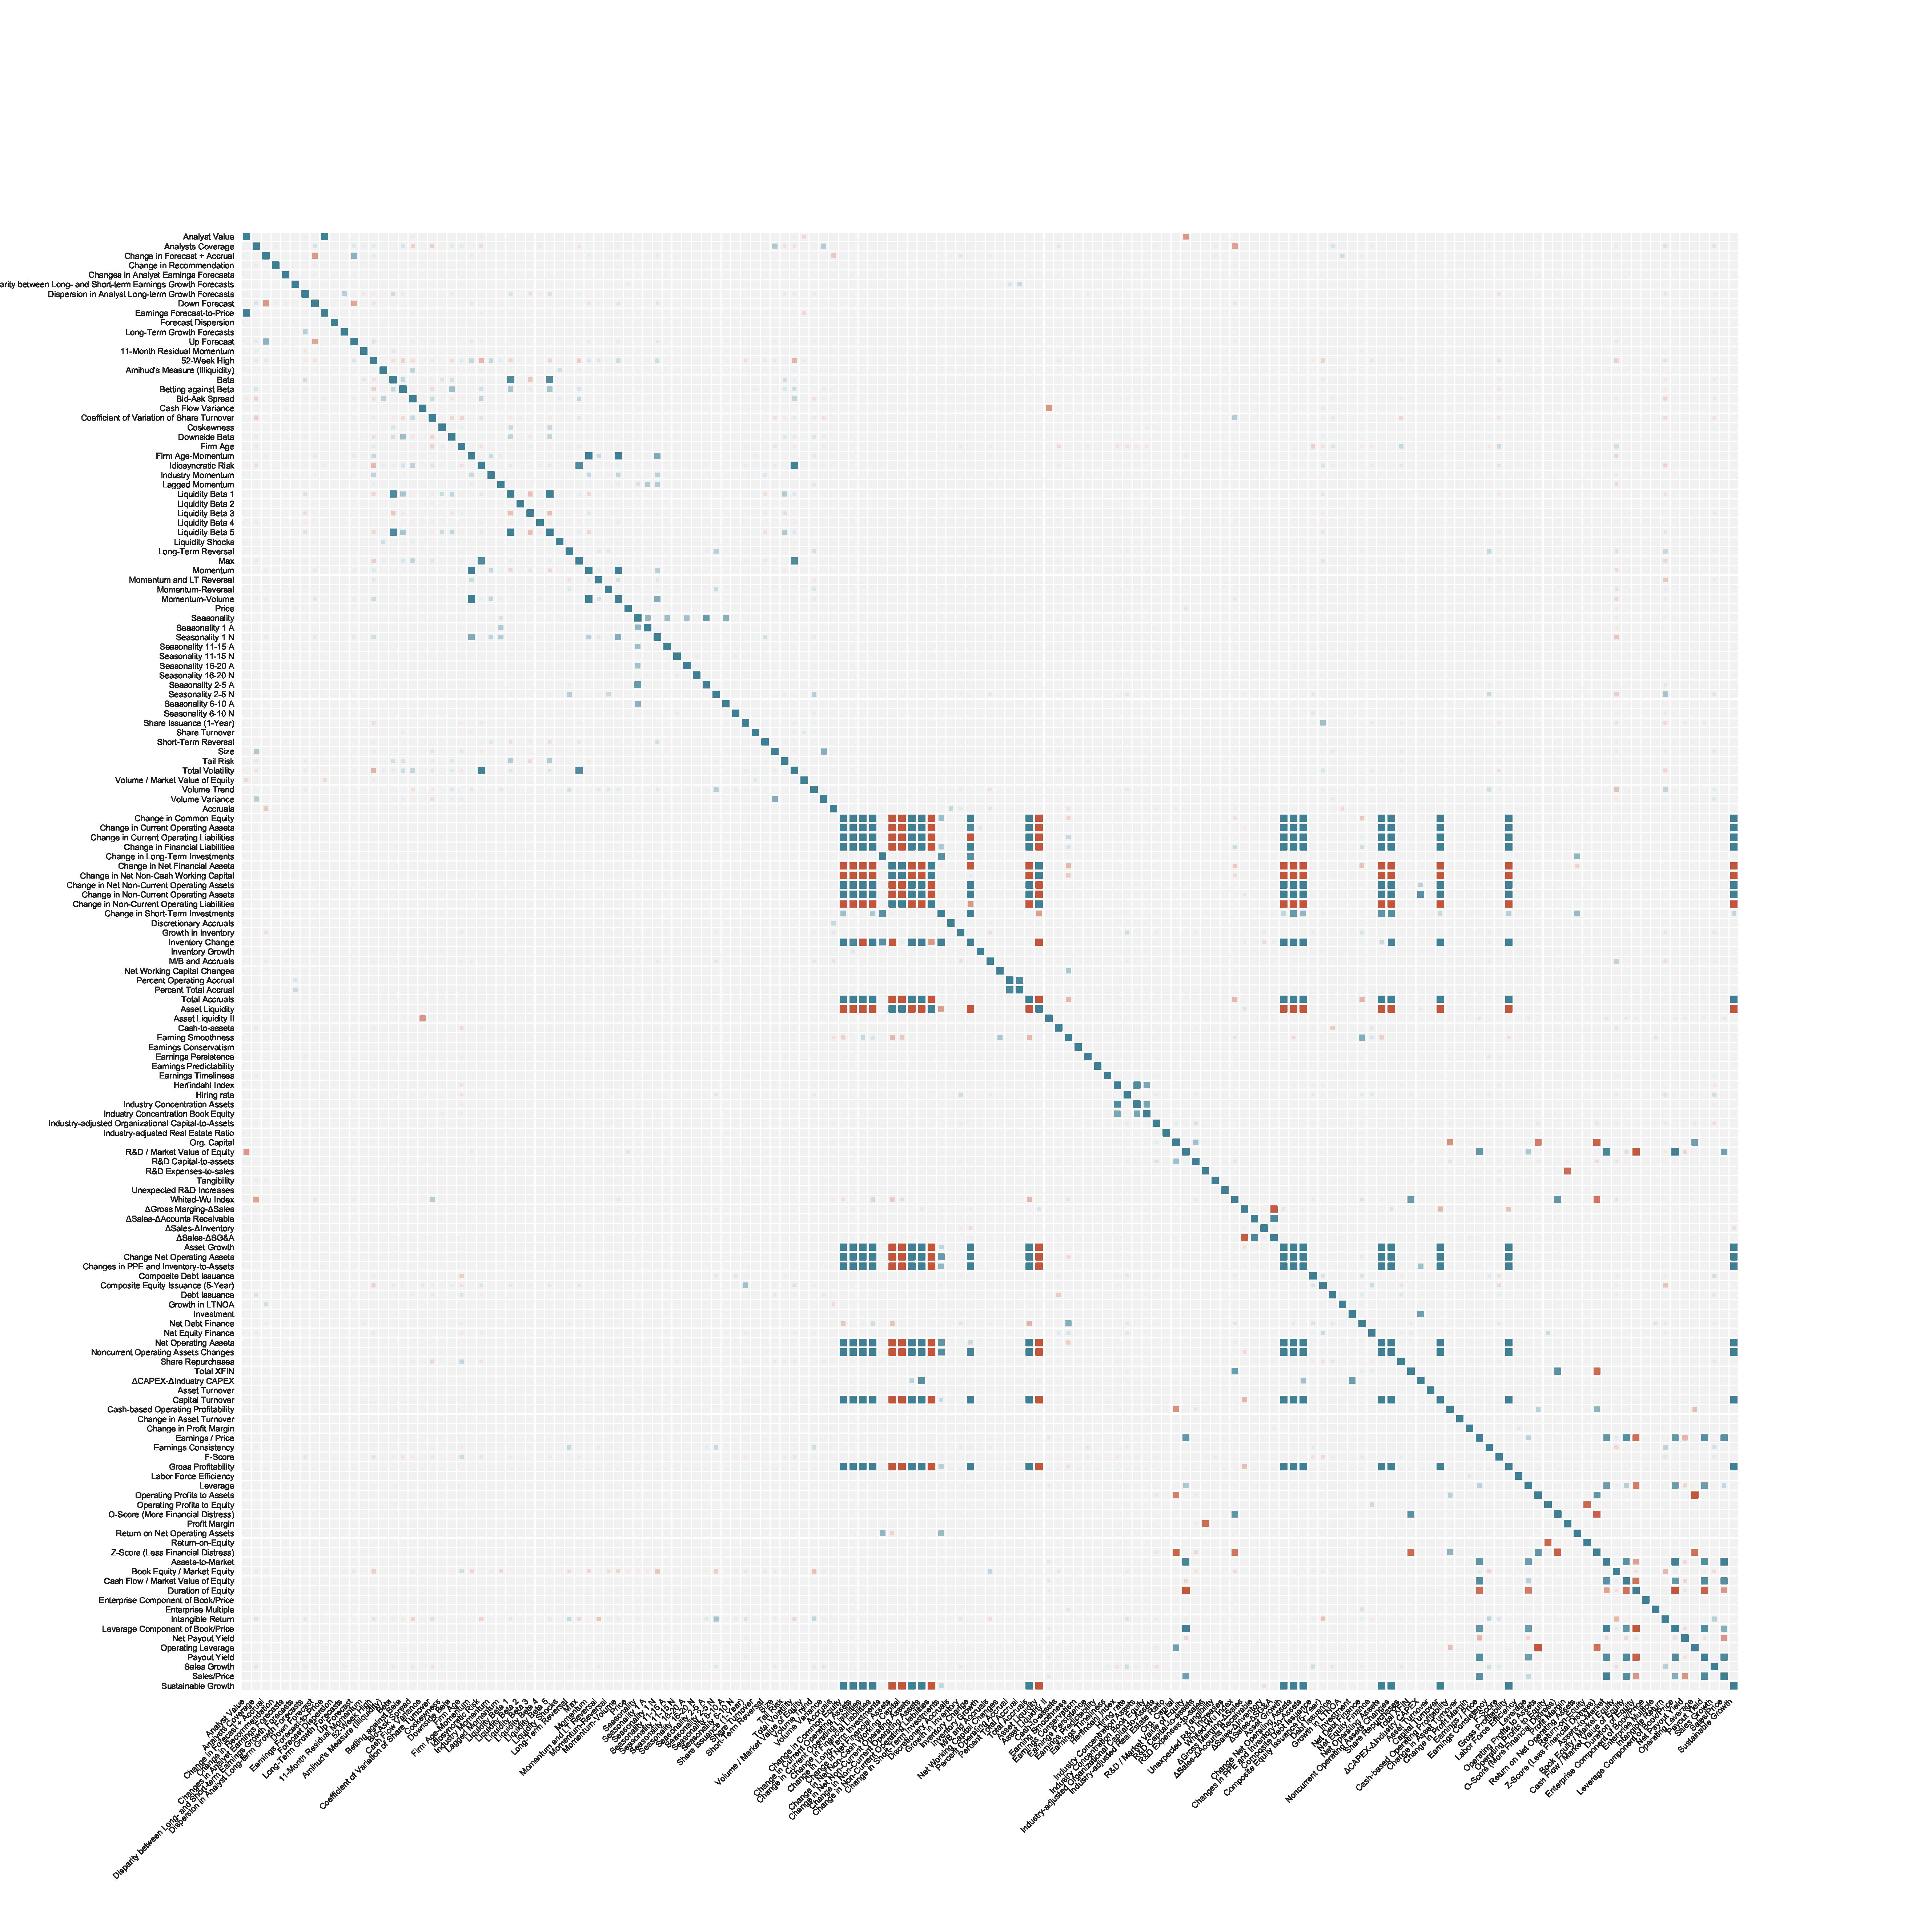
\includegraphics[width=\textwidth,height=\textheight,keepaspectratio]{Figures/corrplot.pdf}
			\caption{Correlation Matrix of the Anomalies}
			\label{fig:corrplot}
		\end{figure}
	\end{center}
	
	
	\begin{center}
		\begin{figure}
			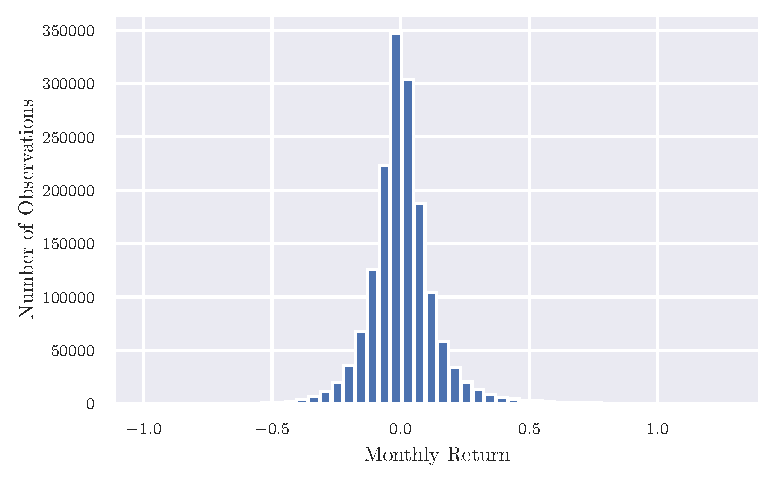
\includegraphics{Figures/hist_returns.pdf}
			\caption{Histogram of Monthly Returns}
			\label{fig:hist_returns}
		\end{figure}
	\end{center}


		
	


